\section{Experiments}
At first, we define a performance measurement in terms of the ideal performance as follows:
\[
P = \sum_i \frac{Number(action_i)}{i}
\]
where we assume that ideal number of actions should be the same as the number of steps. We will use this measurement for scoring each agent.

\subsection{Memoryless Reflex Agent}
In this case, the agent cannot finish the cleaning, which cleaned up $36$ cells in 76 steps. The performance curve is shown in figure \ref{fig:agent1}. The memoryless agent get score of $0.503$.

\begin{figure}[!h]
\centering
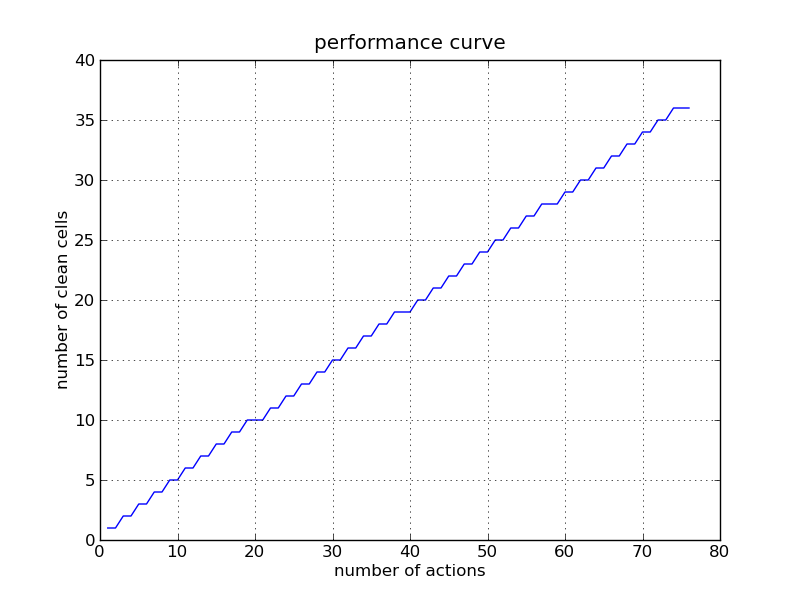
\includegraphics[scale=.35]{img/agent1.png}
\caption{Performance of Memoryless Deterministic Agent}
\label{fig:agent1}
\end{figure}

\subsection{Randomized Reflex Agent}
We run $50$ trials for the randomized reflex agent. The number of actions to take to clean $90\%$ of the room is shown in table \ref{tab:agent2}. We also show the performance curves for each trial in figure \ref{fig:agent2}. The average actions of best 45 trials is $524.96$. The score of this agent is $0.118$. We didn't see extreme case in our experiment, which may always able to choose the right action for making an optimal path. The randomized agent wastes lots of steps to finish the cleaning, but at least it has no limitations, so it is very possible to clean up the room before turning off. This is much better than the memoryless one.

\begin{table}[h]
    \centering
    \begin{tabular}{|l|c|c|c|c|c|c|c|c|c|c|}
        \hline
        trials 1-10 & 495 & 625 & 514 & 647 & 842 & 614 & 550 & 532 & 532 & 924\\ \hline
        trials 11-20 & 510 & 585 & 519 & 616 & 504 & 434 & 477 & 538 & 489 & 479\\ \hline
        trials 21-30 & 385 & 562 & 531 & 591 & 551 & 458 & 515 & 711 & 662 & 439\\ \hline
        trials 31-40 & 461 & 398 & 604 & 601 & 900 & 428 & 507 & 594 & 512 & 735\\ \hline
        trials 41-50 & 572 & 574 & 490 & 498 & 578 & 517 & 380 & 444 & 605 & 506\\ \hline
    \end{tabular}
    \caption{Number of actions to take to clean $90\%$ of the room}\label{tab:agent2}
\end{table}

\begin{figure}[!h]
        \centering
        \subfloat[Number of actions]{
                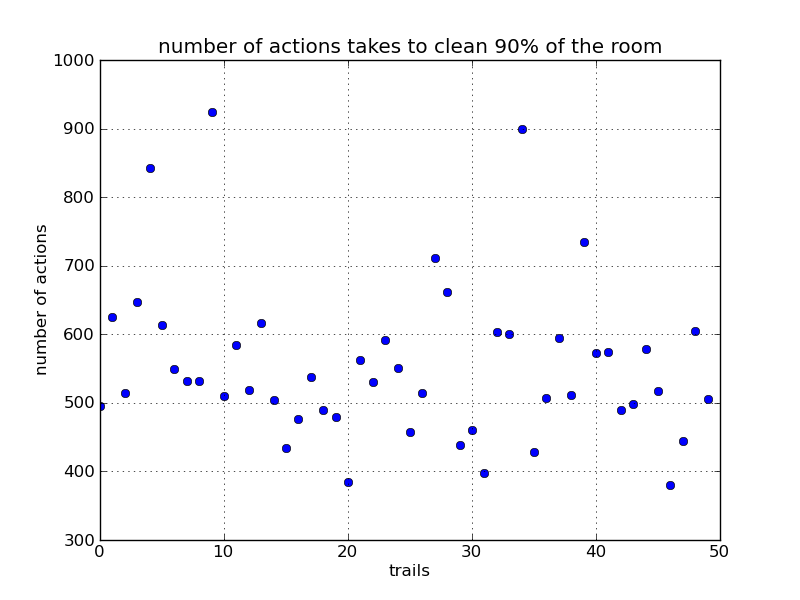
\includegraphics[scale=0.35]{img/num_actions.png}
        }
        \hspace{0.5in}
        \subfloat[Performance curves]{
                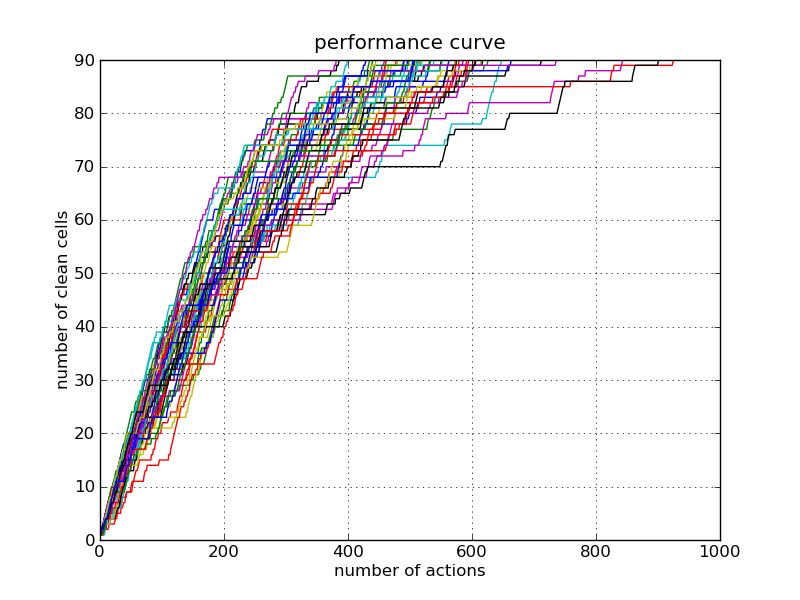
\includegraphics[scale=0.35]{img/rand.png}
        }
        \caption{Performance of randomized reflex agent}\label{fig:agent2}
\end{figure}

\subsection{Deterministic Model-based Agent}

For any $n>0$, $m>0$ and $0\le p \le1$, the agent is able to completely clean the room and shut off itself properly. The algorithm assumes the home cell is always the bottom-left corner of the world and the world is always a rectangular nxm array of cells with walls only at the boundarie of the rectangle. If the home cell is somewhere else, then it may miss cells to the west and south of its starting location. If the world is not rectangular, then it may make a premature assumption that the world is clean or it may navigate incorrectly such that it misses some cells.

For $n=10$, $m=10$ and $p=1.0$ as in the default case, the agent took 230 steps. The model based agent get score of 0.472. We show the performance curve in figure \ref{fig:agent3}.

\begin{figure}[!h]
\centering
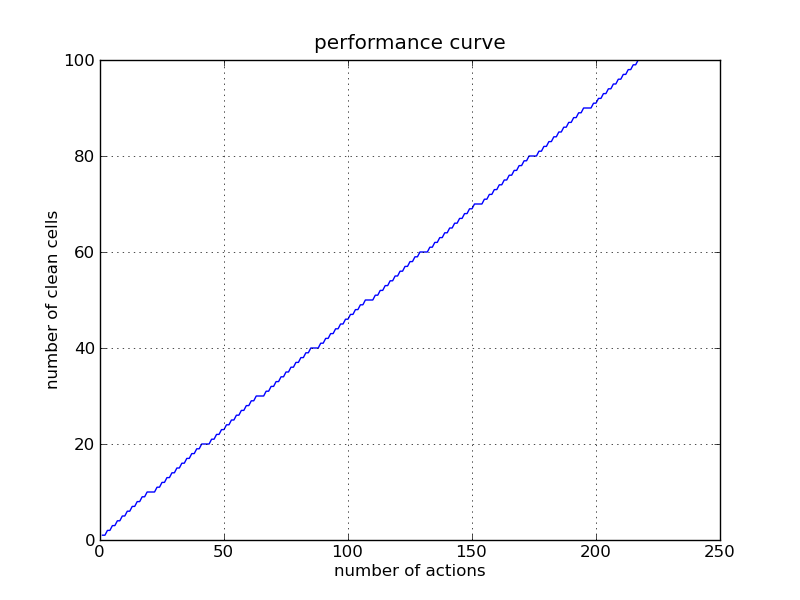
\includegraphics[scale=.35]{img/agent3.png}
\caption{Performance of Model Based Agent}
\label{fig:agent1}
\end{figure}
